% !TeX spellcheck = de_DE
\section{Evolutionäre Algorithmen}
\label{sec:evolutionary_algos}
Für die Optimierung von \ac{KNN} können verschiedene Algorithmen eingesetzt werden. Der in Kapitel \ref{subsec:backprop_algo} vorgestellte Backpropagation Algorithmus ist hierbei nur ein Beispiel. In dieser Arbeit kommt das in Kapitel \ref{sec:neat} vorgestellte Verfahren zum Einsatz, welches der Gruppe der neuroevolutionären Algorithmen zuzuordnen ist, deren Basis sogenannte \acp{EA} sind. Zu diesen gehören eine Vielzahl von unterschiedlichen Verfahren, denen allerdings gemeinsame Grundprinzipien zugrunde liegen.
Ziel der \ac{EA} ist, eine möglichst gute Näherungslösung für ein Optimierungsproblem zu finden. Umgesetzt wird dies mit einer simulierten Evolution, welche durch das biologische Pendant inspiriert ist \cite{weicker2015evolutionare}.

\subsection{Biologische Evolutionäre Konzepte}
\label{subsec:biological_evolution}
Einer der bedeutendsten Wissenschaftler in Bezug auf die Evolutionstheorie ist Charles Darwin, welcher 1859 mit seiner Arbeit \emph{On the Origin of Species by Means of Natural Selection} eine wichtige Grundlage gelegt hat \cite{russell2013kunstliche}. Theoretisch wird bei Betrachtung der Evolution zwischen unbelebten Systemen und lebenden Organismen unterschieden \cite{weicker2015evolutionare}. Da die \ac{EA} von Letzteren inspiriert sind, wird im weiteren Verlauf dieser Arbeit nur auf diese Bezug genommen.
\\\\
Die im weiteren Verlauf der Arbeit vorgestellten \ac{EA} übernehmen aus der Biologie verschiedene Begriffe, wie zum Beispiel Population, Individuum, Genotyp, Phänotyp, Selektion, Rekombination und Mutation. Diese werden im Folgenden aus Sicht des biologischen Vorbilds betrachtet. Die Erklärungen in dieser Arbeit sind stark vereinfacht und es werden zudem ausschließlich die konzeptionellen Prinzipien vorgestellt. Der genaue biologische Ablauf ist für diese Arbeit nicht relevant. Eine Population setzt sich aus vielen unterschiedlichen und unabhängigen Individuen zusammen, welche alle zur selben Art gehören. Eine Art ist hierbei definiert als eine Gruppe von Individuen mit einem gemeinsamen Genpool, die sich untereinander paaren können. Jedes Individuum besitzt ein Genom, welches das genetische Erbgut enthält. Dieses besteht aus mehreren Chromosomen, die wiederum mehrere Gene besitzen \cite{weicker2015evolutionare}. Hierbei kann ein Gen, welches zum Beispiel für die Fell- bzw. Haarfarbe des Individuums verantwortlich ist, verschiedene Werte annehmen. Jede dieser Ausprägungen wird als Allel bezeichnet \cite{weicker2015evolutionare}. Somit ist das Genom der Bauplan für ein Individuum und bestimmt maßgeblich dessen Erscheinungsbild \cite{kirschbaum2008biopsychologie}. Der Phänotyp wird durch das Genom beeinflusst und beschreibt die tatsächlichen, äußerlich feststellbaren Ausprägungen der einzelnen Gene \cite{weicker2015evolutionare}, wobei allerdings auch ein Einfluss der Umwelt auf den Phänotypen möglich ist \cite{kirschbaum2008biopsychologie}. Die Kombination aus Genom und Phänotyp bildet das bereits vorgestellte Individuum. 
\\\\
Nachdem im vorherigen Absatz die grundlegenden Begriffe bezüglich einzelner Individuen erläutert wurden, soll jetzt mit Bezug auf die Evolution die Population als Ganzes betrachtet werden. Die heute existierende Vielfalt an Tier- und Pflanzenarten hat sich über viele Millionen Jahren entwickelt. Der genaue Ursprung der Entstehung erster Lebewesen mit Stoffwechselprozessen ist dennoch unbekannt. Mit Fokus auf die Evolution stellt sich die Frage, wie sich das genetische Material im Laufe der Zeit ändern kann. Hierfür sind fünf Faktoren zu nennen \cite{weicker2015evolutionare}.
\begin{enumerate}
	\item Der erste und wichtigste Faktor sind zufällige Mutationen. Hierbei entstehen beim Vervielfältigen des genetischen Erbguts Fehler, die zu zufälligen Änderungen führen. So kann beispielsweise ein neues Allel entstehen, welches zu einer neuen, bisher nicht vorhandenen Haar- bzw. Fellfarbe führt \cite{weicker2015evolutionare}. 
	
	\item Der zweite Faktor betrifft die Selektion. Damit verschiedene Allele langfristig ähnlich häufig in der Population vorkommen, müssen mehrere der Selektion zuzuordnende Faktoren zutreffen. Als einer dieser Faktoren ist die Überlebenschance der verschiedenen Individuen in der Umwelt, die sogenannte Umweltselektion, anzuführen \cite{weicker2015evolutionare}. Eine auffällige Fellfarbe kann zum Beispiel ein Nachteil sein, da diese von den natürlichen Feinden leichter entdeckt wird. Durch eine höhere Wahrscheinlichkeit, gefressen zu werden, haben diese Individuen eine geringere Chance zur Fortpflanzung und somit ist es möglich, dass das genetische Material verloren geht. Zuletzt hat nicht nur die Umweltselektion einen Einfluss auf die Anzahl der Nachkommen, sondern auch die erfolgreiche Partnersuche sowie die Fortpflanzungsrate \cite{weicker2015evolutionare}.
	
	\item Besonders in kleinen Populationen kann der Tod einzelner Individuen große Auswirkungen auf das Verhältnis der unterschiedlichen Allele haben. Hierbei können durch Zufall einzelne Allele komplett verloren gehen, wodurch nachfolgende Generationen potenziell stark beeinflusst sind. In diesem Fall spricht man vom sogenannten Gendrift. Der Effekt auf größere Populationen ist allerdings zu vernachlässigen \cite{weicker2015evolutionare}.
	
	\item Wie bereits beschrieben, sollen sich Individuen einer Art fortpflanzen können. Doch es kommt auch vor, dass Individuen einer Art abwandern und sich an zwei räumlich getrennten Orten weiterentwickeln. Einer Zuwanderung ebendieser unterschiedlich weiterentwickelten Teilpopulationen zu einem späteren Zeitpunkt kann eine maßgebliche Veränderung durch die neu entwickelten Gene folgen. Dieser Effekt wird auch Genfluss genannt \cite{weicker2015evolutionare}.
	
	\item Der letzte Faktor ist die Rekombination, die bezüglich der biologischen Evolution den Vorgang der sexuellen Paarung zweier Individuen beschreibt, infolgedessen ein oder mehrere Nachkommen entstehen. Dabei wird das Ergbut für diese aus einer Kombination der Elterngenome erstellt. Somit handelt es sich aus Sicht der klassischen Evolutionslehre nicht um einen Evolutionsfaktor, da nur Bekanntes neu kombiniert wird und keine neuen Gene oder Allele entstehen. Dennoch wird die Rekombination heute meist als Evolutionsfaktor kategorisiert. Grund hierfür ist, dass die einzelnen Gene nicht, wie lange in der Populationsgenetik angenommen, komplett unabhängig voneinander, sondern stattdessen stark vernetzt sind und viel Einfluss aufeinander haben. So können auch bei der Kombination von bekannten Genotypen neue phänotypische Eigenschaften entstehen \cite{weicker2015evolutionare}.
\end{enumerate}
Durch die vorgestellten Arten der Evolution kann sich eine Population verschiedensten Umweltsituationen anpassen und gegenüber konkurrierenden Arten behaupten. Bakterien, welche Resistenzen gegen bestimmte Antibiotika entwickeln, fungieren an dieser Stelle als eingängiges Beispiel. Während die Resistenz anfänglich nur im Genotyp weniger Individuen enthalten ist, wird diese aufgrund der hohe Verbreitung von Bakterien schnell an Nachkommen weitergegeben und ist nach kurzer Zeit in der gesamten Population vorhanden.
 
\subsection{Evolutionäre Algorithmen}
\label{subsec:evolutionary_algorithm}
Im vorherigen Kapitel ist die biologische Evolution vorgestellt, durch die eine Vielzahl von unterschiedlichen Lebensformen aufgrund einer sehr guten Anpassung an ihre jeweilige Umwelt entstanden ist. Da dieses Vorgehen in der Biologie sehr erfolgreich ist, wurden schon im Jahr 1950 erste Versuche durchgeführt, dies auf Computersysteme zu übertragen. Hierbei wird eine bedeutend vereinfachte künstliche Evolution mit dem Ziel simuliert, ein Optimierungsproblem zu lösen \cite{weicker2015evolutionare}. Heute gibt es eine Vielzahl von verschiedenen Algorithmen, die unterschiedliche Aspekte der Evolution imitieren. Im Folgenden werden die Grundkomponenten vorgestellt und verschiedene beispielhafte Umsetzungsmöglichkeiten aufgezeigt.

\subsubsection{Genotyp und Phänotyp}
Wie bei der biologischen Evolution gibt es bei den \ac{EA} Individuen, welche durch einen Genotypen und Phänotypen definiert sind \cite{weicker2015evolutionare}. Das Genom enthält alle Informationen, die nötig sind, um den Phänotypen des Individuums zu erstellen. Die eigentliche Form des Phänotyps ist abhängig vom gegebenen Optimierungsproblem und kann je nach Einsatzszenario unterschiedlich umgesetzt sein \cite{rothlauf2006representation}. Die Repräsentation des Genoms ist in vielen klassischen Algorithmen binär. In diesen Fällen wird das Genom durch einen Vektor $x$ von der Länge $l$ repräsentiert, welcher nur aus den Werten $0$ und $1$ besteht, sodass $x= (x_1, x_2, ..., x_l) \in \{0, 1\}^l$ gilt \cite{rothlauf2006representation}. Der Vektor kann auch natürliche, ganze oder rationale Zahlen enthalten, sollte die vorhergehende Art der Kodierung nicht ausreichend sein \cite{rothlauf2006representation}. Grundsätzlich sind diese Arten der Repräsentationen nur als Beispiele zu verstehen. Jeder Algorithmus kann die Repräsentation der Genome anpassen, sodass es dem Verfahren zuträglich ist. Die in dieser Arbeit verwendete Kodierung ist in Kapitel \ref{subsec:neat_encoding} vorgestellt. 

\subsubsection{Optimierungsproblem}
\label{subsub:optimzation_problem}
Wie bereits beschrieben, ist es Ziel von \ac{EA}, Optimierungsprobleme zu lösen. Diese können aus vielen verschiedenen Bereichen wie Forschung, Wirtschaft sowie Industrie kommen \cite{weicker2015evolutionare} und unterschiedliche Anforderungen haben. Grundsätzlich besteht jedes Optimierungsproblem aus einem dreier Tupel $(\Omega, f, \succ)$ \cite{weicker2015evolutionare}. Die Variable $\Omega$ repräsentiert dabei den Suchraum, also jeden möglichen Lösungsansatz. Dieser wird typischerweise mit einem Individuum und dessen Genom bzw. Phänotyp getestet. Die Funktion $f$ ist definiert als $f: \Omega \rightarrow \mathbb{R}$, sie bewertet jeden Lösungsansatz aus dem Suchraum und weist diesem einen reellen Wert zu, welcher auch als Güte- bzw. Fitnesswert bezeichnet wird \cite{weicker2015evolutionare}. Der letzte Teil des Optimierungsproblems ist eine Vergleichsrelation $\succ \in \{<, >\}$, welche angibt, ob es Ziel ist, ein Minimum oder Maximum in der Fitnessfunktion zu finden \cite{weicker2015evolutionare}. Im Kontext von \ac{EA} wird meist das Maximum gesucht, so auch in dieser Arbeit. Daher wird im Weiteren stets angenommen, dass die Maximierung des erreichten Fitnesswertes das Ziel ist.
\\\\
Bei allen Optimierungsproblemen ist die Fitnessfunktion ein elementarer Bestandteil. Nur diese Funktion gibt dem Algorithmus ein Feedback, wie gut oder schlecht eine Lösung ist. Mithilfe dieser Funktion muss jeder \ac{EA} ableiten, in welche Richtung eine Optimierung sich entwickeln soll, um möglichst effizient eine Lösung zu finden \cite{weicker2015evolutionare}. Aus diesem Grund ist die erste Anforderung an eine solche Funktion, dass sie keine absolute, sondern eine graduelle Bewertung der verschiedenen Lösungsansätze bietet \cite{weicker2015evolutionare}. Beispiel für eine absolute Bewertung ist die Ausgabe des Wertes $1$ durch die Fitnessfunktion bei Lösung des Optimierungsproblems, andernfalls die des Wertes $0$. In diesem Fall kann nicht festgestellt werden, welche Änderungen der Suchparameter erfolgversprechend sind, somit ist es auch nicht möglich, diese gezielt zu ändern. Infolgedessen müssen mehr Lösungsansätze aus dem Suchraum getestet werden, was den Rechenaufwand und die benötigte Zeit erhöht. Des Weiteren muss die Fitnessfunktion möglichst vollständig die Ziele des Optimierungsproblems abbilden. Andernfalls kann zwar durch den Algorithmus das Ergebnis der Fitnessfunktion maximiert werden, die hierdurch gefundene Lösung enthält jedoch nicht unbedingt die vom Anwender gewünschten Eigenschaften \cite{weicker2015evolutionare}.

\subsubsection{Ablauf evolutionärer Algorithmen}
Aus den vorherigen Kapiteln ist ersichtlich, dass Individuen aus einem Genotyp sowie Phänotyp bestehen und dass diese versuchen, ein Optimierungsproblem zu lösen. Die Aufgabe eines \ac{EA} ist, die Individuen langfristig so anzupassen, dass sie bessere Fitnesswerte im Optimierungsproblem erzielen und dementsprechend eine gute Lösung finden. Hierzu werden die aus der Biologie bekannten Faktoren Selektion, Rekombination und Mutation eingesetzt. Bevor in den weiteren Kapiteln verschiedene Umsetzungen beispielhaft vorgestellt werden, wird in diesem Abschnitt der grundlegende Ablauf von \ac{EA} erläutert.
\begin{figure}[h]
	\centering
	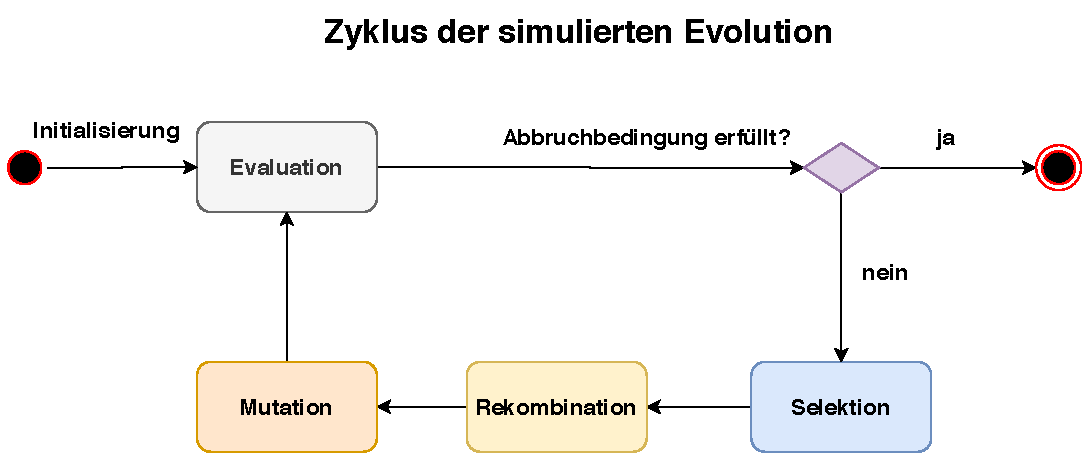
\includegraphics[width=0.9\textwidth]{./img/ea_basics/ea_cycle.pdf} 
	\caption{Schematische Darstellung des Zyklus bei der simulierten Evolution}
	\label{fig:ea_cycle}
\end{figure}
\\\ \noindent
Abbildung \ref{fig:ea_cycle} zeigt den beispielhaften Ablauf von \ac{EA}, wobei die Phasen Evaluation, Selektion, Mutation und Rekombination die größte Bedeutung haben. Bevor der eigentliche Programmablauf starten kann, muss eine erste initiale Population erzeugt werden. Wie in der biologischen Evolution, besteht sie auch aus mehreren unabhängigen Individuen \cite{rothlauf2006representation}. Im Gegensatz zum biologischen Vorbild verwenden die meisten Algorithmen ein feste Populationsgröße, da ansonsten die später benötigte Evaluationszeit und der damit verbundene Rechenaufwand stark ansteigen kann \cite{rothlauf2006representation}. Die den Individuen zugehörigen Genome werden zufällig erstellt \cite{weicker2015evolutionare}, wobei je nach Algorithmus verschiedene Zufallsverteilungen genutzt werden können.
\\\\
Danach beginnt die Evaluationsphase mit der initialen Population \cite{rothlauf2006representation}. Hierfür wird der Phänotyp für jedes Individuum mit dem entsprechenden Genom gebildet. Jeder dieser Phänotypen stellt eine mögliche Lösung für das gegebene Optimierungsproblem dar. Wie im vorherigen Kapitel beschrieben, muss dieses eine Fitnessfunktion enthalten, mit welcher jeder Phänotyp bewertet wird. An dieser Stelle ist erneut hervorzuheben, dass die Gesamtheit aller Gene den Phänotypen bestimmt und daher keine Bewertung einzelner Gene möglich ist \cite{rothlauf2006representation}. Die Evaluationsphase endet, wenn für alle Phänotypen ein Fitnesswert ermittelt ist. Der nächste Schritt ist die Überprüfung einer Abbruchbedingung. Trifft diese zu, wird die Ausführung des Algorithmus abgebrochen und das Genom des besten Individuums als Ergebnis zurückgegeben \cite{weicker2015evolutionare}. Je nach Umsetzung der Abbruchbedingung kann zum Beispiel überprüft werden, ob ein gewisser Fitnesswert erreicht und somit eine Lösung mit der gewünschten Genauigkeit bzw. Korrektheit gefunden wurde oder ob eine vorher definierte maximale Ausführungszeit überschritten ist.
\\\\
Die Abbruchbedingung wird zu Beginn mit sehr hoher Wahrscheinlichkeit nicht erfüllt sein, da die Genome nur zufällig erstellt sind und bisher kein Lernprozess stattgefunden hat. In diesem Fall werden die Phasen Selektion, Rekombination und Mutation durchgeführt \cite{rothlauf2006representation}. Diese werden in den folgenden Kapiteln ausführlich erläutert, daher wird in diesem Abschnitt nur ein kurzer Überblick gegeben. In der ersten Phase, der Selektion, wird auf Basis des erhaltenen Fitnesswertes für jedes Individuum festgelegt, ob und wie viele Nachkommen dieses erzeugen darf \cite{weicker2015evolutionare}. Bei der Rekombination werden die tatsächlichen Nachkommen erzeugt. Typischerweise werden zwei, in manchen Fällen auch mehr Individuen als Elterngenome ausgewählt und gekreuzt. Dieser Vorgang sieht die Vermischung des genetischen Materials, welches in den Elterngenomen enthalten ist, sowie die Übertragung auf das neue erstellte Kind-Individuum vor. Das Ziel dieser Operation ist, dass das Kind immer einen Teil der Gene von beiden Eltern erhält und somit auch Eigenschaften von beiden vereint. Langfristig sollen sich durch ein solches Verfahren nur die besten Gene durchsetzen \cite{weicker2015evolutionare}. 
Die letzte Phase ist die Mutation. In diesem Schritt besteht für jedes neu erstellte Individuum die Wahrscheinlichkeit, dass ein kleiner Teil des Genoms zufällig abgeändert wird \cite{rojas1996neural}. Die Art der Mutation ist hierbei abhängig von der Umsetzung des Genotypen und vom Algorithmus. Bezüglich der drei Phasen muss verdeutlicht werden, dass die Selektion auf Basis des Phänotypen mit dem Fitnesswert erfolgt, die Rekombination und Mutation hingegen auf Basis des Genotypen. Somit können keine Eigenschaften, die im Phänotyp gespeichert sind, auf die Nachkommen übertragen werden \cite{rothlauf2006representation}.
\\\\
Nach Abschluss dieser drei Phasen sind die neuen Individuen fertig erstellt. Da, wie bereits in diesem Kapitel beschrieben, die Populationsgröße meistens begrenzt ist, wird an dieser Stelle typischerweise die Elterngeneration komplett entfernt und durch dieselbe Anzahl an Nachkommen ersetzt \cite{weicker2015evolutionare}. Allerdings gibt es auch andere Ansätze, bei denen nicht so viele neue Individuen gleichzeitig erstellt werden und diese dann direkt in die bestehende Population integriert werden können \cite{stanley2005real}. Die neue Population mit den neuen Individuen durchläuft dieselben Schritte wie die vorherige Population. Ein kompletter Durchlauf des vorgestellten Zyklus wird als eine Generation bezeichnet \cite{weicker2015evolutionare}. Häufig wird die neu erstellte Population daher auch als neue Generation bezeichnet. 

\subsubsection{Selektion}
\label{subsubsec:ea_selection}
Bei \ac{EA} werden viele Individuen eingesetzt, um verschiedene Lösungsansätze gleichzeitig zu betrachten. In der Phase der Selektion wird bestimmt, welche Individuen als Elternteil für die nächste Generation ausgewählt werden und wie viele Nachkommen ihnen zustehen. Bei einem solchen Auswahlverfahren ist zwischen zwei grundlegenden Umsetzungen zu unterscheiden. Die Anzahl der Nachkommen der Individuen einer Generation ist entweder abhängig vom erreichten Fitnesswert oder unabhängig, sodass dann allen Individuen dieselbe Anzahl an Nachkommen zugewiesen wird. Typischerweise wird die erste Variante in \ac{EA} verwendet, welche auch als fitnessproportionale Selektion bezeichnet wird. Die zweite Variante erzeugt keinen Selektionsdruck, da die Individuen unabhängig von ihrer Leistung Nachkommen zugewiesen bekommen. Bei der ersten Variante werden Individuen mit höheren Fitnesswerten mit dem Ziel bevorzugt, dass sich die positiven Eigenschaften der erfolgreichen Individuen durchsetzen und schlechte aussterben. Dennoch ist es nicht das Ziel, nur die allerbesten Genome als Elternteile auszuwählen. Wäre dies der Fall, würde die Population sehr schnell konvergieren, ihre Vielfalt verlieren und nur noch ähnliche Lösungsansätze bieten, womit das Finden von neuen, unbekannten, aber eventuell besseren Lösungsansätzen unwahrscheinlich ist \cite{weicker2015evolutionare}. 
\\\\
Der genaue Selektionsvorgang, wie er im Algorithmus dieser Arbeit umgesetzt ist, wird in Kapitel \ref{subsec:neat_species} erläutert. Im Folgenden werden zwei verschiedene Varianten der fitnessproportionalen Verfahren vorgestellt, die in anderen Algorithmen als Selektionsfunktion verwendet werden. Wie bereits allgemeingültig beschrieben, wird die Anzahl an Nachkommen durch den jeweils erreichten Fitnesswert beeinflusst \cite{weicker2015evolutionare}.

\begin{enumerate}
	\item \textbf{Probabilistische Selektion}:\\
	Eine der bekanntesten Umsetzungen ist die probabilistische Selektion, welche grundsätzlich einfach zu implementieren ist. Im ersten Schritt werden die erreichten Fitnesswerte $f$ der einzelnen Individuen $i$ in der Population $P$ aufsummiert. Im zweiten Schritt wird für jedes Individuum $j$ die Wahrscheinlichkeit $Pr[j]$ berechnet, welche angibt, wie groß die Chance ist, dass dieses als Elternteil ausgewählt wird. Sie ergibt sich aus dem Quotienten des erhaltenen Fitnesswertes und der berechneten Summe, sodass $Pr[j]=\frac{f_j}{\sum_{i \in P}f_i}$ gilt. Diese Art der Selektion ist in vielen Anwendungsfällen sehr erfolgreich. Allerdings kann es vorkommen, dass bei sehr hohen Fitnesswerten die prozentualen Unterschiede zwischen guten und schlechten Individuen sehr gering sind und infolgedessen der Selektionsvorteil für gute Lösungen niedrig ist. Ein möglicher Lösungsansatz besteht in der Skalierung der Fitnesswerte, sodass auch bei hohen Durchschnittswerten kleine Steigerungen einen evolutionären Vorteil bieten \cite{weicker2015evolutionare}. Ein weiterer Lösungsansatz ist die Verwendung der rangbasierten Selektion, welche im Folgenden vorgestellt wird.
	
	\item  \textbf{Rangbasierte Selektion}:\\
	Bei der rangbasierten Selektion ist der tatsächlich erhaltene Fitnesswert nicht von Bedeutung. Die Individuen werden bezüglich ihrer Fitness geordnet. Das beste Individuum erhält die größte, das schlechteste die geringste Wahrscheinlichkeit, als Elternteil ausgewählt zu werden \cite{weicker2015evolutionare}. 
\end{enumerate}
Sind die Wahrscheinlichkeiten für alle Individuen berechnet, ist im letzten Schritt festzulegen, welche Genome tatsächlich als Elternteile ausgewählt werden und wie viele Nachkommen diese erzeugen. Bei der fitnessproportionalen Selektion wird hierfür ein Zufallsgenerator benötigt, welcher basierend auf den Wahrscheinlichkeiten die Elterngenome auswählt. Dass diesem Verfahren ein Nachteil entsteht, wird darin deutlich, dass obwohl das beste Individuum die höchste Wahrscheinlichkeit hat, als Elternteil ausgewählt zu werden, es auf Basis des Zufalls dazu kommen kann, dass dieses nicht verwendet wird. Da typischerweise die Population am Ende des Evolutionszyklus ersetzt wird, würde das genetische Material dieses Individuums verloren gehen \cite{weicker2015evolutionare}. Um einen solchen Verlust zu verhindern, kann bei der Selektion zusätzlich ein sogenannter Elitismus verwendet werden. Hierbei wird typischerweise der Genotyp des besten Individuums ausgewählt, kopiert und unverändert wieder in die nächste Generation eingesetzt \cite{such2017deep}. Zu beachten ist allerdings, dass im weiteren Verlauf ein Nachkomme weniger produziert wird, um eine konstante Populationsgröße zu garantieren. 

\subsubsection{Rekombination}
\label{subsubsec:ea_recombination}
Die Phase der Rekombination wird auch als \emph{crossover} bezeichnet und findet nach der Selektion statt. Die Aufgabe dieser ist, die ausgewählten Elternindividuen zu nutzen, um neue Nachkommen zu erstellen. Typischerweise werden zwei, in einigen Fällen auch mehr Elternteile kombiniert, um mindestens ein Kind-Individuum zu erzeugen \cite{weicker2015evolutionare}. Die Rekombination gilt als eine der wichtigsten Phasen, da die Nachkommen tendenziell bessere Ergebnisse erzielen sollen als die Elternteile \cite{russell2013kunstliche}. Wie auch bei anderen Phasen der \ac{EA} gibt es verschiedene Arten der Umsetzung, die als kombinierende, interpolierende und extrapolierende Selektion zu bezeichnen sind \cite{weicker2015evolutionare}. Die bekannteste dieser drei Varianten ist die kombinierende Selektion, welche sowohl in dieser Arbeit als auch in vielen anderen Algorithmen verwendet wird. Die beiden Alternativen werden bedeutend seltener gewählt und sind auch in der Literatur oft nicht erwähnt. Dennoch werden im Folgenden alle Varianten kurz vorgestellt.
\\\\
Die kombinierende Rekombination ist stark von der Biologie inspiriert. Bei diesem Vorgang werden die Genome der Elternteile zuerst nebeneinander aufgereiht. Im zweiten Schritt wird zufällig entschieden, welcher Abschnitt von welchem Elternteil für das Genom des Nachkommens verwendet werden soll \cite{weicker2015evolutionare}. Der Vorteil dieses Verfahrens ist, dass große Informationsblöcke, welche unabhängig voneinander optimiert wurden und sinnvolle Funktionen realisieren, von den Elternteilen geerbt werden können \cite{russell2013kunstliche}. Der aus der Rekombination entstehende Nachkomme kann hierdurch einen Vorteil bei der Evaluation besitzen und letztendlich eine bessere Lösung für das Optimierungsproblem bieten. Da diese Art der Rekombination keine neuen Gene erstellt bzw. bestehende modifiziert, ist der Erfolg abhängig davon, ob die Population eine gewisse Diversität bietet, sodass bei der Rekombination tatsächlich verschiedene Gene kombiniert werden können \cite{weicker2015evolutionare}. In der praktischen Umsetzung muss zuletzt noch entschieden werden, an welchen Stellen eine Rekombination möglich ist \cite{rojas1996neural}. Bei der uniformen Rekombination wird für jedes einzelne Gen unabhängig von den anderen zufällig entschieden, von welchem Elternteil es übernommen wird \cite{weicker2015evolutionare}. Bei anderen Umsetzungen hingegen werden die Gene zuerst in Gruppen eingeteilt, woraufhin zwischen diesen zufällig entschieden wird.
\\\\
Bei der interpolierenden Rekombination werden die einzelnen Gene nicht direkt von einem Elternteil übernommen, stattdessen werden sie gemischt, sodass ein neuer Wert entsteht, der sich zwischen den Werten der Elternteile befindet. Im Gegensatz zur kombinierenden Rekombination, welche versucht, die Diversität zu erhalten, wird diese hierbei deutlich verringert. Aus diesem Grund ist es notwendig, dass zu Beginn eine Population mit einer großen Diversität vorhanden ist, sodass der Suchraum  des Optimierungsproblems ausgiebig überprüft wird. Ein Beispiel für eine solche technische Umsetzung ist die sogenannte arithmetische Rekombination, welche für reellwertig repräsentierte Genome verwendet werden kann. Angenommen, die Werte $A_i$ und $B_i$ repräsentieren die Gene der Eltern $A$ und $B$, dann wird für jedes Gen $i$ eine Zufallszahl $u$ zwischen $0$ und $1$ bestimmt. Das Gen $C_i$ des Nachkommens $C$ berechnet sich durch $C_i=u \cdot A_i + (1-u) \cdot B_i$ \cite{weicker2015evolutionare}.
\\\\
Die letzte Variante ist die extrapolierende Rekombination, welche mit mehreren Elternteilen versucht, eine Prognose darüber abzugeben, wo im Suchraum eine Steigerung des Fitnesswertes möglich ist, und dementsprechend versucht, die Genome der Nachkommen zu ändern. Somit kann diese Art der Rekombination auch neue Gene erstellen. Die Nachteile eines solchen Verfahrens sind darin zu verdeutlichen, dass es, um eine Prognose abzugeben, erstens nötig ist, ein Grundwissen über den Suchraum zu haben, und zweitens die Gefahr besteht, dass die vorgegebene Richtung nicht korrekt und die Funktion danach nicht fähig ist, eine systematische Suche durchzuführen \cite{weicker2015evolutionare}.   

\subsubsection{Mutation}
\label{subsubsec:ea_mutation}
Der letzte Schritt, bevor die bestehende Population durch die neu erstellten Individuen ersetzt wird, ist typischerweise die Mutation. Allerdings ist die Funktionsweise und Relevanz dieser Phase stark abhängig von der verwendeten Kodierung und dem eigentlichen Algorithmus \cite{weicker2015evolutionare}. So wird beispielsweise in Quelle \cite{such2017deep} gar keine Rekombination verwendet und die Optimierung wird nur mithilfe der Mutation umgesetzt, während in anderen Quellen wie in \cite{zoller2007kunstliche} diese Phase als untergeordnet und nur selten einzusetzen beschrieben wird.
\\\\
Wird die Mutation häufig verwendet, erfüllt sie zwei Aufgaben. Das erste Ziel ist die Feinabstimmung der einzelnen Individuen, sodass das Optimum der Fitnessfunktion so genau wie möglich erreicht werden kann. Das zweite Ziel ist die Erforschung des Suchraums, welche stichprobenartig durchgeführt wird, um ein besseres Optimum zu finden \cite{weicker2015evolutionare}.  Wird die Mutation selten eingesetzt, müssen die Feinabstimmung und Erforschung durch andere Komponenten, wie zum Beispiel die Rekombination, durchgeführt werden. In diesem Fall ist es das Ziel der Mutation, neue Diversität in die Population zu bringen bzw. diese zu erhalten \cite{weicker2015evolutionare}. Denn wie bereits im vorherigen Kapitel beschrieben, ist vor allem bei der viel verwendeten Rekombination die Diversität sehr wichtig, wobei sie allerdings meist durch die Rekombination selbst verringert wird.
\\\\
Da die Umsetzung der Mutation sowohl von der Kodierung als auch vom Algorithmus abhängig ist, gibt es keine Empfehlungen, welche Implementierung besonders viele Vorteile bietet. Im Folgenden werden zwei mögliche Beispiele vorgestellt, wobei das erste für Individuen mit einer binären und das zweite für diejenigen Individuen mit einer reellwertigen Repräsentation angewendet werden kann \cite{weicker2015evolutionare}. Die einfachste Mutation ist die Binär-Mutation, welche für Genome mit einer binären Repräsentation verwendet werden kann. Bei der Mutation wird für jedes Bit eine Zufallszahl $u$ zwischen $0$ und $1$ bestimmt. Ist diese kleiner als die festgelegte Mutationswahrscheinlichkeit $p_m$, wird das Bit invertiert. Sind die Individuen durch reellwertige Zahlen repräsentiert, ist die sogenannte Gauss-Mutation eine mögliche Umsetzung. Bei dieser wird für jedes Gen eine Zufallszahl basierend auf einer Gauss-Verteilung gewählt, wobei eine zuvor festgelegte Standardabweichung $\sigma$ die Verteilung beeinflusst. Die hierdurch erhaltene Zahl wird auf den bereits bestehenden Wert addiert \cite{weicker2015evolutionare}.

\subsection{Neuroevolution}
\label{subsec:neuroevolution}
Wie im vorherigen Kapitel erläutert, sind \ac{EA} Verfahren, um möglichst gute Näherungslösungen für verschiedene Optimierungsprobleme zu finden. Für die in Kapitel \ref{sec:neuroal_networks} vorgestellten \ac{KNN} wird ein Verfahren benötigt, welches die verschiedenen anpassbaren Parameter optimiert. Es ist dementsprechend möglich, die evolutionären Prinzipien zur Optimierung von \ac{KNN} einzusetzen. Dies wird als Neuroevolution bezeichnet \cite{meisner2009neurostrategies}. Algorithmen dieser Art sind somit eine Alternative zu den klassischen Verfahren, zu denen auch der Backpropagation Algorithmus zählt \cite{whitley1993genetic}. Im Vergleich zu diesem haben neuroevolutionäre Verfahren sowohl Vor- als auch Nachteile, welche ausführlich in Kapitel \ref{subsec:comparision_neuroevoltion} beschrieben werden. Dennoch soll ein großer Vorteil bereits hier genannt sein. Das Ziel der meisten neuroevolutionären Algorithmen ist das Optimieren von Verbindungsgewichten und Schwellwerten. Einige Verfahren versuchen, zusätzlich die Struktur bzw. Topologie des \ac{KNN} zu optimieren, sodass diese nicht mehr manuell durch einen Entwickler festgelegt werden muss. Wie in Kapitel \ref{subsec:network_structures} beschrieben, ist die Topologie ein maßgeblicher Faktor für die erfolgreiche Lösung des Optimierungsproblems. Diese Algorithmen werden als \ac{TWEANN} Verfahren bezeichnet \cite{stanley2002evolving}. 
\\\\
Auch der in Kapitel \ref{sec:neat} vorgestellte Algorithmus optimiert sowohl die Topologie als auch die Gewichte eines \ac{KNN}. Im Folgenden sollen sowohl der Ablauf von neuroevolutionären Algorithmen als auch die Besonderheiten erläutert sowie zuletzt Vor- und Nachteile näher verdeutlicht werden.

\subsubsection{Ablauf der Neuroevolution}
Der grundsätzliche Ablauf von neuroevolutionären Algorithmen ist nahezu identisch zu den klassischen \ac{EA}. Auch bei diesen gibt es eine Population, welche aus verschiedenen Individuen besteht, die einen Genotyp und Phänotyp besitzen. Letzteres besteht bei der Neuroevolution aus einem \ac{KNN}, welches durch den Genotyp kodiert ist. Auch die Definition des Optimierungsproblems ist identisch zur Erklärung in Kapitel \ref{subsub:optimzation_problem}. Ein Phänotyp, in diesem Fall ein \ac{KNN}, versucht, das Optimierungsproblem zu lösen und erhält hierdurch einen Fitnesswert, welcher angibt, wie gut oder schlecht die Lösung ist. Wenn dieser Wert für alle Mitglieder einer Population berechnet ist, beginnen die Phasen Selektion, Rekombination und Mutation. Hierdurch werden neue Individuen mit neuen Genotypen und Phänotypen erstellt, welche dann die vorherige Population ersetzen. Dieser Zyklus wird so oft wiederholt, bis eine Abbruchbedingung erreicht ist. Natürlich ist es möglich, dass die praktische Umsetzung je nach Algorithmus angepasst wird. Einige grundlegende Anpassungen werden in den folgenden Abschnitten erläutert. Wie die angesprochenen Aspekte von dem in dieser Arbeit verwendeten Algorithmus umgesetzt werden, wird in Kapitel \ref{sec:neat} erläutert.

\subsubsection{Genotyp und Phänotyp}
Eine Komponente, die auf jeden Fall angepasst werden muss, ist der Genotyp, welcher alle optimierbaren Parameter für den Phänotypen kodieren muss. Typischerweise umfasst die Kodierung die Struktur des Netzes, die Gewichte der Verbindungen sowie die Schwellwerte \cite{stanley2002evolving}. Die Propagierungs-, Aktivierungs- und Ausgabefunktion müssen nur enthalten sein, wenn diese ebenfalls durch den \ac{EA} angepasst werden. Hierdurch ergibt sich die Frage, wie diese Informationen im Genom zu kodieren sind, sodass auch eine erfolgreiche Durchführung der Rekombinations- und Mutationsphase möglich ist. 
\\\\
Grundsätzlich gibt es zwei verschiedene Kodierungansätze, die ein Algorithmus verwenden kann. Diese werden als direkte und indirekte Kodierung bezeichnet. Bei einer direkten Kodierung wird im Genom jede einzelne Verbindung und jedes Neuron explizit spezifiziert, sodass diese einfach im Phänotyp übernommen werden können. Diese Art der Kodierung wird häufig verwendet, da sie einfach zu implementieren ist und auch die Rekombination und Mutation damit gut umsetzbar sind. Die indirekte Kodierung als Alternative spezifiziert Regeln, die angeben, wie aus einem Genom ein \ac{KNN} erstellt werden soll. Als vorteilhaft ist zu verdeutlichen, dass nicht jede Verbindung und jedes Neuron einzeln kodiert werden muss, die Repräsentation dementsprechend kompakter ist und dadurch weniger Rechenkapazität zur Speicherung benötigt wird \cite{stanley2002evolving}. Nachteil von dieser Methode ist, dass die Rekombination und Mutation komplexer umzusetzen sind. Im Folgenden wird nur noch auf die direkte Kodierung Bezug genommen, da sie in dieser Arbeit verwendet wird.
\\\\
Theoretisch kann für eine direkte Kodierung des Genoms, wie bei klassischen \ac{EA}, eine binäre Repräsentation verwendet werden. Umsetzbar ist dies mit einer Matrix, welche für jede mögliche Verbindung angibt, ob diese besteht oder nicht. Allerdings hat eine solche Kodierung einige Nachteile, weswegen sie für diesen Anwendungsfall eher ungeeignet ist. Ein Grund ist der benötigte Speicherplatz für ein einzelnes Genom. Die Matrix enthält für ein \ac{KNN} mit $n$ Neuronen insgesamt $n^2$ Einträge für die möglichen Verbindungen \cite{stanley2002evolving}. Für große \ac{KNN} skaliert dieser Ansatz schlecht.
\\\\
Alternativ hierzu ist eine Graphen-Kodierung, welche auch von vielen \ac{TWEANN} Algorithmen verwendet wird. Eine mögliche Umsetzung mit einer zweiteiligen Kodierung liefern \citeauthor{pujol1998evolving} in ihrer Arbeit \cite{pujol1998evolving}. Der erste Teil beschreibt die Struktur des Graphen bzw. des \ac{KNN}, während der zweite Teil ein linearer Vektor ist, welcher die Neuronen und Verbindungen enthält. Kapitel \ref{subsec:neat_encoding} geht ausführlich auf die in dieser Arbeit zur Anwendung kommende Variante ein.

\subsubsection{Rekombination}
\label{subsubsec}
Chronologisch gesehen findet die Selektion vor der Rekombination statt. Da sie aber analog zur Selektion in den \ac{EA} stattfindet, liegt der Fokus im Folgenden direkt auf der Rekombination. Prinzipiell ist das Verfahren ähnlich der Beschreibung in Kapitel \ref{subsubsec:ea_recombination}. Die Selektion hat zwei Elterngenome ausgewählt und diese werden im Rahmen der Rekombination zu einem neuen Genom kombiniert. Typischerweise wird bei diesem Vorgang zufällig entschieden, welche Verbindung von welchem Elternteil übernommen werden soll. Das Ziel ist, ein \ac{KNN} zu erzeugen, welches in den meisten Fällen die positiven Eigenschaften der Eltern erbt und somit insgesamt besser wird. Eine Schwierigkeit, die hierbei in Bezug auf Neuroevolution entstehen kann, wird als das \emph{Competing Conventions} Problem bezeichnet \cite{stanley2002evolving}.
\\\\ % TODO Comepting Conevntions ABbildung da
Der Begriff \emph{Competing Conventions} beschreibt ein Phänomen, bei dem mehrere \ac{KNN} dieselbe Lösung für ein Optimierungsproblem bieten, die Repräsentationen der Genome dennoch unterschiedlich sind. Ein solches Beispiel ist in Abbildung (TODO Abbildung) dargestellt. Die beiden \ac{KNN} besitzen je drei verdeckte Neuronen (4, 5, 6) mit den dazugehörigen Verbindungen in den Farben blau (B), rot (R) und grün (G). Die tatsächlichen Gewichte sind hierbei nicht von Interesse und werden deshalb für eine bessere Übersichtlichkeit durch die Farben repräsentiert. Das erste \ac{KNN} kann beispielsweise durch den Vektor (B, R, G), das zweite durch den Vektor  (G, R, B) kodiert werden. Es besteht die Annahme, dass in der Kodierung die einzelnen Gewichte für alle Verbindungen enthalten sind. \\\\
Wie in der Abbildung zu erkennen ist, sind die beiden \ac{KNN} symmetrisch und produzieren infolgedessen für dieselbe Eingabe auch dasselbe Ergebnis, während sich die Genotypen allerdings bezüglich ihrer Kodierung unterscheiden. Werden diese beiden \ac{KNN} durch die Selektion ausgewählt, um einen Nachkommen zu erzeugen, wird das \emph{Competing Conventions} Phänomen mit hoher Wahrscheinlichkeit zu einem Problem führen, das im Nachfolgenden beschreiben ist. 
\\\\
Wie bei traditionellen \ac{EA} wird auch bei der Neuroevolution typischerweise zufällig entschieden, von welchem Elternteil welches Gen übernommen werden soll. Angenommen, es werden die ersten beiden Gene vom linken Elternteil und das letzte Gen vom rechten Elternteil übernommen, dann ist das daraus resultierende neue Genom mit (B, R, B) kodiert. Es ist ersichtlich, dass bei diesem Vorgang ein Drittel der Informationen verloren gegangen sind bzw. nicht vererbt wurden. Dies ist in den meisten Fällen ein großes Problem, da der fehlende Teil mit hoher Wahrscheinlichkeit einen notwendigen Beitrag für einen Lösungsansatz kodiert hat, der das Elterngenom erfolgreich gemacht hat. Aus diesem Grund wird das neu erstellte Individuum wahrscheinlich weniger erfolgreich sein als seine Elternindividuen, erhält einen dementsprechend niedrigeren Fitnesswert und wird letztendlich aussterben \cite{stanley2002evolving}. Tritt dieser Fall nur bei einem einzelnen Genom in einer Population auf, sind die Auswirkungen meist zu vernachlässigen. Allerdings gibt es für ein \ac{KNN} mit $x$ verdeckten Neuronen in einer Schicht $x!$ verschiedene Kombinationsmöglichkeit, dieselbe Lösung durch unterschiedliche Genome zu repräsentieren \cite{stanley2002evolving}. Somit ist die Wahrscheinlichkeit, dass das \emph{Competing Conventions} Problem eintritt, relativ hoch. Die Folge ist, dass entweder viel Rechenzeit für Genome verwendet wird, die mit hoher Wahrscheinlichkeit keine besseren Lösungen bereitstellen und dadurch das Optimierungsverfahren bedeutend länger dauert, oder dass das Verfahren scheitert, da keine ausreichend gute Lösung gefunden werden kann. 
% Viele fälle, mehr rechenzeit oder unmöglich 
\\\\
Bei den \ac{TWEANN} Algorithmen ist das \emph{Competing Conventions} Problem noch größer \cite{stanley2002evolving}. Wie bereits beschrieben, versuchen diese, auch die Struktur des \ac{KNN} zu optimieren und können im Zuge dessen neue Neuronen und Verbindungen hinzufügen. Im nächsten Kapitel wird hierauf genauer eingegangen. An dieser Stelle sei allerdings vorweggenommen, dass im Laufe des Optimierungsverfahrens eine Population mit unterschiedlichen Strukturen und Topologien entstehen kann. Es stellt sich die Frage, wie  unterschiedliche \ac{KNN} rekombiniert werden können, wenn die Genome unterschiedlich groß sind und nicht zuzuordnen ist, welche Gene der Eltern rekombiniert werden können. Hierbei handelt es sich um die schwierigste Form des \emph{Competing Conventions} Problems \cite{stanley2002evolving}. Die Lösung des Problems durch den in dieser Arbeit verwendeten Algorithmus ist in Kapitel \ref{sec:neat} erläutert.

\subsubsection{Mutation}
\label{subsubsec:mutation}
Bei neuroevolutionäre Algorithmen wird die Mutation in der Regel häufig eingesetzt. Die erste zweier möglicher Arten wendet die Mutation ausschließlich auf die Verbindungsgewichte und Schwellwerte an. Hierfür kann die bereits in Kapitel \ref{subsubsec:ea_mutation} vorgestellte Gauss-Mutation verwendet werden, wobei der erhaltene Zufallswert auf das Gewicht bzw. den Schwellwert addiert wird \cite{mcintyre_neatpython}. Die zweite Art, die als strukturelle Mutation bezeichnet wird, verändert die Topologie, worin deutlich wird, dass sie ausschließlich für \ac{TWEANN} Verfahren benötigt wird, welche dem \ac{KNN} neue Neuronen und Verbindungen hinzufügen können \cite{stanley2002evolving}.
\\\\
Das eigentliche Hinzufügen von neuen Strukturen ist schon durch die Verknüpfung zweier bisher unverbundener Neuronen durch eine neue Verbindung mit einem zufälligen Gewicht jederzeit zu bewerkstelligen. Allerdings wird hierdurch der Fitnesswert in den meisten Fällen initial sinken, da es unwahrscheinlich ist, dass eine zufällige Struktur eine nützliche Funktionalität oder Teillösung bietet. Infolgedessen sinkt auch die Chance, dass das Genom bei der Selektion in der nächsten Generation als Elternteil ausgewählt und die neue Struktur an die Nachkommen vererbt wird. So kommt es häufig vor, dass die strukturellen Innovationen direkt in der nächsten Generation verloren gehen, obwohl sie zum Teil für eine erfolgreiche Lösung notwendig wären. Die daraus resultierende Herausforderung für \ac{TWEANN} Verfahren besteht darin, neue Innovationen am Anfang zu schützen, sodass der Algorithmus diese optimieren kann. Nur so ist es möglich, neue Strukturen langfristig in die Population zu integrieren \cite{stanley2002evolving}.
\\\\
Eine mögliche Lösung der beschriebenen Problematik ist in der Arbeit von \citeauthor{angeline1994gnarl} vorgestellt. Hierbei werden neue Neuronen ohne jegliche Verbindungen in das \ac{KNN} eingefügt, während neue Verbindungen initial das Gewicht $0$ haben. Die so hinzugefügten Strukturen haben anfänglich keinen Effekt auf das \ac{KNN}. Ziel hiervon ist, dass der Fitnesswert nicht absinkt und sich die Strukturen im Laufe von mehreren Generationen selbstständig entwickeln \cite{angeline1994gnarl}. Diese Umsetzung ist allerdings nicht ideal, da die Strukturen unter Umständen nicht richtig in das \ac{KNN} integriert werden, aber dennoch die benötigte Rechenkapazität erhöhen \cite{stanley2002evolving}.
\\\\
Der in Kapitel \ref{sec:neat} vorgestellte Algorithmus verfolgt einen anderen Ansatz, bei dem ähnliche \ac{KNN} einer Spezies zugeordnet werden. Ein Individuum soll nicht mehr mit der ganzen Population konkurrieren, sondern nur mit denen seiner Spezies. Dies wird auch als \emph{niching} bezeichnet. Eine neue, große strukturelle Mutation wird einer neuen Spezies zugeordnet und kann innerhalb dieser entwickelt und optimiert werden. Zur Bestimmung, ob ein Genom einer Spezies zugehörig ist, wird eine Kompatibilitätsfunktion benötigt. Die Umsetzung von dieser Funktion wird durch das \emph{Competing Conventions} Problem erschwert \cite{stanley2002evolving}, worauf in Kapitel \ref{subsec:neat_species} genauer eingegangen wird.
 
\subsubsection{Initiale Population}
Die initiale Population der ersten Generation enthält zufällig erstellte \ac{KNN}. Die benötigten Verbindungsgewichte und Schwellwerte werden häufig mithilfe einer Gauss-Verteilung gewählt \cite{mcintyre_neatpython}. Die Wahl der initialen Topologie kann sich jedoch stark unterscheiden. Bei den neuroevolutionären Algorithmen, welche ausschließlich die Verbindungsgewichte und Schwellwerte optimieren, wird diese zu Beginn einmalig für die gesamte Laufzeit des Verfahrens für alle \ac{KNN} festgelegt.
\\\\
Bei den \ac{TWEANN} Algorithmen hingegen können verschiedene initiale Topologien verwendet werden, welche unter anderem die Laufzeit des Algorithmus stark beeinflussen können. Viele dieser Algorithmen erstellen zu Beginn verschiedene zufällig gewählte Topologien, mit dem Ziel, Diversität in die Population zu bringen. Ein Nachteil dieser Strategie ist die potenzielle Entstehung ungeeigneter \ac{KNN}, bei denen beispielsweise nicht alle Eingabeneuronen mit allen Ausgabeneuronen verbunden sind. Zudem ergibt sich in diesem Fall noch ein weiteres Problem \cite{stanley2002evolving}. Grundsätzlich ist es sinnvoll, die kleinst mögliche Struktur zu wählen, die dennoch einen mit größeren \ac{KNN} vergleichbaren Fitnesswert für ein Optimierungsproblem erzielt \cite{zhang1993evolving}. Diese hat im Vergleich zu größeren Strukturen weniger anpassbare Parameter, was generell die benötigte Optimierungszeit reduziert. Wenn die Topologien allerdings zufällig erstellt sind, werden hierbei viele unnötige Strukturen enthalten sein, was zu einem größeren Suchraum führt und die Laufzeit des Optimierungsverfahrens erhöht \cite{stanley2002evolving}. 
\\\\
In einem solchen Fall muss das Optimierungsverfahren versuchen, die Größe des \ac{KNN} aktiv zu minimieren. Ein Ansatz diesbezüglich ist in der Arbeit von \citeauthor{zhang1993evolving} beschrieben, in welcher die Größe des \ac{KNN} den Fitnesswert beeinflusst. In diesem Fall haben kleinere \ac{KNN} bei gleicher Performance hinsichtlich des Optimierungsproblems einen größeren Fitnesswert und dementsprechend eine größere Chance, bei der Selektion ausgewählt zu werden. Das endgültige Ziel hierbei ist, dass langfristig nur die benötigten Strukturen erhalten bleiben \cite{zhang1993evolving}. Zusätzlich kann die Entscheidung, wie viel Einfluss die Größe des \ac{KNN} tatsächlich auf den Fitnesswert haben soll, in der Praxis schwierig sein \cite{stanley2002evolving}.
\\\\
Eine weiterer Lösungsansatz ist das Starten mit einer minimalen Struktur, sodass das \ac{KNN} zu Beginn keine verdeckten Neuronen besitzt. Neue Strukturen werden nur integriert, wenn sie einen höheren Fitnesswert ermöglichen. Der Vorteil dieser Strategie ist, dass keine Rechenzeit verwendet werden muss, um unnötige Strukturen zu entfernen, und dass zusätzlich die Anzahl an anzupassenden Parametern gering ist \cite{stanley2002evolving}.

\subsection{Neuroevolution im Vergleich}
\label{subsec:comparision_neuroevoltion}
Grundsätzlich wächst das Interesse an neuroevolutionären Algorithmen und in vielen Anwendungsfällen sind bereits auch im Vergleich mit anderen Ansätzen gute Ergebnisse erzielt worden \cite{meisner2009neurostrategies}. Dennoch werden Algorithmen dieser Art oft mit Skepsis betrachtet und weniger eingesetzt als gradientenbasierte Verfahren wie beispielsweise der Backpropagation Algorithmus. Daher wird in vielen Arbeiten ein Vergleich zwischen auf Gradienten basierenden Verfahren und neuroevolutionären Algorithmen gezogen. In diesem Kapitel werden einige Vor- und Nachteile vorgestellt, die häufig im Zusammenhang mit entsprechenden Vergleichen genannt werden \cite{rojas1996neural, meisner2009neurostrategies, such2017deep, whitley1993genetic}.
\\\\
Für einen aussagekräftigen Vergleich müssen neuroevolutionäre Algorithmen zuvor noch einer Art des Lernens, deren Varianten in Kapitel \ref{subsec:learning_in_neural_networks} vorgestellt sind, zugeordnet werden, da sich die Aufgaben und Anwendungsfälle in diesen stark unterscheiden können. Neuroevolutionäre Algorithmen sind dem bestärkenden Lernen zuzuordnen \cite{whitley1993genetic}. Ein häufig genannter Grund dieser Zuordnung ist die Vergleichbarkeit des Fitnesswertes bei neuroevolutionären Algorithmen mit dem insgesamt erhaltenen \emph{reward}, dessen Maximierung das Ziel des bestärkenden Lernens ist \cite{such2017deep}. Darüber hinaus haben \citeauthor{sutton2018reinforcement} bestärkendes Lernen in ihrer Arbeit als eine Methode beschrieben, welche \ac{MDP} Probleme lösen kann. Das in Kapitel \ref{subsec:learning_in_neural_networks} vorstellte \ac{MDP} Problem beschreibt die Interaktion zwischen einem Agenten und seiner Umgebung. Hierbei kann der Agent als ein Individuum von neuroevolutionären Algorithmen und die Umgebung als Optimierungsproblem betrachtet werden. 
\\\\
Ein grundsätzlicher Vorteil von neuroevolutionären Algorithmen ist, dass durch die vielen Individuen unterschiedliche Lösungsansätze überprüft werden können. Dies ermöglicht es den Algorithmen, lokale Optima zu überwinden und die Suche nach dem globalen Optimum weiter fortzuführen \cite{rojas1996neural}, was für gradientenbasierte Verfahren schwierig sein kann. Ein weiterer Vorteil ist darin aufzuzeigen, dass bei neuroevolutionären Algorithmen keine Gradienten berechnet werden müssen \cite{rojas1996neural}, da dies aufwendig sein kann. Für die neuroevolutionären Algorithmen wird lediglich die Fitnessfunktion benötigt. 
\\\\
Allerdings kann diese einfache Art der Evaluation durch die Fitnessfunktion zum Nachteil werden, wenn das Optimierungsproblem bzw. die Umwelt verschiedene Startzustände hat. So kann ein Individuum mit einem schlechten Lösungsansatz durch Zufall einen einfachen Startzustand erhalten und so unter Umständen einen höheren Fitnesswert erzielen als ein besserer Lösungsansatz eines anderen Individuums, welchem ein ungünstiger Startzustand zugewiesen wird. Als mögliche Konsequenz aus dem vorher beschriebenen Szenario können einige gute Individuen an der Weiterentwicklung der Population unbeteiligt sein, da sie aufgrund eines geringen Fitnesswerts nicht bei der Selektion ausgewählt werden und verloren gehen. Die Fitnessfunktion wird in einem solchen Fall als verrauscht oder \emph{noisy} bezeichnet. Ein möglicher Lösungsansatz ist, allen Individuen immer denselben Startzustand zuzuweisen. Eine daraus entstehende Problematik lässt sich insofern erkennen, dass das Lernen ebendieser Individuen ausschließlich auf den ausgewählten Startzustand beschränkt ist, was sie für andere und vor allem ungünstigere Startzustände mit hoher Wahrscheinlichkeit unbrauchbar macht. Zu umgehen ist diese Problematik durch die Testung aller Individuen mit verschiedenen Startzuständen und einer 
Akkumulierung der einzelnen Fitnesswerte \cite{whitley1993genetic}. Nachteil dieses Ansatzes ist, dass sich die Laufzeit linear erhöht je mehr verschiedene Startzustände getestet werden.
\\\\
Ein weiteres Problem von neuroevolutionären Algorithmen ist die Laufzeit, da das Entwickeln unterschiedlicher Lösungen durch verschiedene Individuen viel Rechenzeit benötigt \cite{rojas1996neural}. Für eine Population mit beispielsweise $1000$ Mitgliedern werden pro Generation $1000$ \ac{KNN} erstellt, von denen mit jedem versucht wird, das Optimierungsproblem zu lösen. Die hierfür benötigte Laufzeit ist oft höher als bei gradientenbasierten Verfahren, bei welchen ein einziges \ac{KNN} evaluiert werden muss \cite{whitley1993genetic}. Gleichzeitig kann dies aber auch ein großer Vorteil für neuroevolutionäre Algorithmen sein, wie unter anderem in Quelle \cite{such2017deep} gezeigt ist. Da die einzelnen Individuen unabhängig voneinander sind, lässt sich ihre Evaluation gut parallelisieren \cite{rojas1996neural}, sodass eine Reduzierung der Ausführungszeit unabhängig von Limitierungen einzelner Prozessoren möglich ist \cite{schleuter1991explicit}. Das bedeutet, dass im Gegensatz zu sequentiellen Programmen, bei denen die Ausführungszeit nur durch einen schnelleren Prozessor gesenkt werden kann, die Laufzeit von parallelisierbaren Algorithmen auch durch das Hinzufügen von weiteren Prozessoren verringert werden kann. Dies ist in vielen Fällen einfacher und kostengünstiger umzusetzen.

% Struktur  
% 0 Vortgeil: TWEANN Algorithmen entwicklen Struktur
% 1 Vorteil, Suchen an vielen verschiedenen Punkten im Lösungsraum, Wahrscheinlich nicht stuck an lokalen Optimmum
% 2. Vorteil: Es werden keine Gradienten benötigt, welche teilweise schwer zu berechnen sind sondern nr die Fitnessfunktion
% 1. Nachtei: Verrasuchte Fitnessfunktino
% 2. Nachteil: Viele KNN benötigten viel Rechenzeit, EA eher langsam
% 3. Vorteil: Gut parallelisierbar


% Neuro Networks A Systematic Introduction
% •	Genetic algorithms can be used when no information is available about the gradient of the function at the evaluated points. The function itself does not need to be continuous or differentiable. Genetic algorithms can still achieve good results even in cases in which the function has several local minima or maxima
% •	These properties of genetic algorithms have their price: unlike traditional random search, the function is not examined at a single place, constructing a possible path to the local maximum or minimum, but many different places are considered simultaneously. The function must be calculated for all elements of the population.
% •	However, compared to other stochastic methods genetic algorithms have the advantage that they can be parallelized with little effort. Since the calculations of the function on all points of a population are independent from each other, they can be carried out in several processors
% •	advantage that they do not necessarily remain trapped in a suboptimal local maximum or minimum of the target function
% •	genetic algorithm can move away from a local maximum or minimum if the population finds better function values in other areas of the definition domain
% o	Genetic algorithms offer some interesting properties to offset their high computational cost. We can mention at least three of them: a) GAs explore the domain of definition of the target function at many points and can thus escape from local minima or maxima
% o	he function to be optimized does not need to be given in a closed analytic form – if the process being analyzed is too complex to describe in formulas, the elements of 
% o	) since evaluation of the target function is independent for each element of the population, the parallelization of the GA is quite straightforward. A population can be distributed on several processors and the selection process carried out in parallel
% •	The problem of symmetries (Competing Conventions Problem)
% •	One field in which GAs seem to be a very appropriate search method is game theory
% o	Mathematicians then ask what is the optimal strategy, that is, how can a player maximize his pay-off. In many cases the cumulative effect of the pay-off function cannot be expressed analytically and the only possibility is to actually play the game and compare the results using different strategies


% Deep Neuroevolution: Genetic Algorithms are a Competitive Alternative for Training Deep Neural Networks for Reinforcement Learning
% •	Evolution strategies (ES) can rival backprop-based algorithms such as Q-learning and policy 
% •	At a high level, an RL problem challenges an agent to maximize some notion of cumulative reward (e.g. total, or discounted) without supervision as to how to accomplish that goal 
% •	hey found that this algorithm, which we will refer to simply as evolution strategies (ES), is competitive with DQN and A3C on difficult RL benchmark problems, with much faster training times (i.e. faster wall-clock time when many CPUs are available) due to better parallelization (Salimans et al., 2017). 
% •	One motivation for choosing ES versus Q-learning and policy gradient methods is its faster wall-clock time with distributed computation, owing to better parallelization 
%o	A reason GA might outperform gradient-based methods is if local optima are present, as it can jump over them in the parameter space, whereas a gradient method cannot


% Genetic Reinforcment Learning for Neurocontrol Problems
% Genetic Algorithms can produce roughly competetive results as the standard back prop ago
% Domains where EA can make uniqze contribution -> No Derivate function, Gradient not available or costly to obtain
% EA sind eine ARt des RL Learnings
% Resulting search time is signigicantly lower than back Prop
% One Problem Noisy fitness function?

% Neuroevolution strategies for episodic reinforcement learning
% Growing INterest in NeuroEvolution -> sind Reinforcment Learning Technik, Gute Performance im Vergleich zu anderen Alternativen


% -----------------------------------------------------------

% Evolutionäre ALgos mit Neuronalen Netzen, Prinzipien mit Phasne gleich


% ERgen immer mehr aufmerksam, Gute Ergebnisse
% One Problem, slower then backpropagation with lager NN, One problem symmetric representations
% Calculation of gradiant expensive in recurrent NM

%Can achive better wall clock time, Can be used if gradients are hard to calculate, ) GAs explore the domain of definition of the %target function at many points and can thus escape from local minima or maxima, einfache bewertung mit fitness funktion, 
%•	These properties of genetic algorithms have their price: unlike traditional random search, the function is not examined at a %single place, constructing a possible path to the local maximum or minimum, but many different places are considered %simultaneously. The function must be calculated for all elements of the population.
%•	However, compared to other stochastic methods genetic algorithms have the advantage that they can be parallelized with little %effort. Since the calculations of the function on all points of a population are independent from each other, they can be carried %out in several processors
%•	advantage that they do not necessarily remain trapped in a suboptimal local maximum or minimum of the target function
%•	genetic algorithm can move away from a local maximum or minimum if the population finds better function values in other areas %of the definition domain
% Probabilistische Strahlsuche ?

% Obwol Diversität gut und wichtig für Entdecken des Suchrausm, oft Problem da Unvollstände NAchkommen erzeugt werden